\chapter{Descripción del Trabajo}
\label{cap:descripcionTrabajo}
En este capitulo se describe el framework de enemigos creado, mediante el diseño de componentes más sencillos. 
Primero se describirá el contexto y por tanto la utilidad de la herramienta, aquí se detallaran juegos analizados y características en común. Después se explicará que elementos la componen y por último se detallarán algunos ejemplos de uso. \\
\section{Contexto}
\subsection{Enemigo}
Los enemigos son entidades programadas para oponerse al jugador y crear desafíos dentro del juego. Generalmente, tienen características, comportamientos y habilidades diseñadas para interactuar con las mecánicas del juego y contribuir a la experiencia del jugador. \\

\section{Composición}
En este trabajo, se ha decidido entender como enemigo a cualquier entidad que pueda repercutir de forma negativa en el jugador. Esto significa que no se limita el concepto de enemigo a figuras típicas, como monstruos o soldados hostiles, sino que se amplía su definición a toda entidad que suponga un riesgo, dificultad o amenaza para el progreso o el bienestar del jugador dentro del juego, como pueden ser pinchos, lava o gotas de ácido.
Además separamos cada enemigo por comportamientos diferentes, implicando que elementos que clásica mente aparecen en conjunto, como la tubería y la gota de ácido o la bala y el pistolero, serán considerados como  dos enemigos distintos.\\

\subsection{Máquina de estados finita}

La Máquina de Estados Finita (FSM, Finite State Machine) es el núcleo de la lógica que define el comportamiento de los enemigos en nuestro diseño de videojuegos. Cada enemigo tiene su propia FSM, configurada específicamente para representar sus patrones de acciones, reacciones y relaciones en el juego. La FSM organiza el comportamiento de los enemigos mediante estados y transiciones:
Los estados agrupan las acciones que el enemigo puede realizar en un momento dado.
Las transiciones permiten cambiar de un estado a otro y son activadas por sensores.
Estos conceptos (estados, sensores y eventos) se desarrollan con mayor detalle en los apartados siguientes.

El objeto enemigo se define mediante una máquina de estados finita y un script que contiene información relevante. A continuación, se describen ambos conceptos y sus propiedades.\\
\begin{figure}[h]
	\centering
	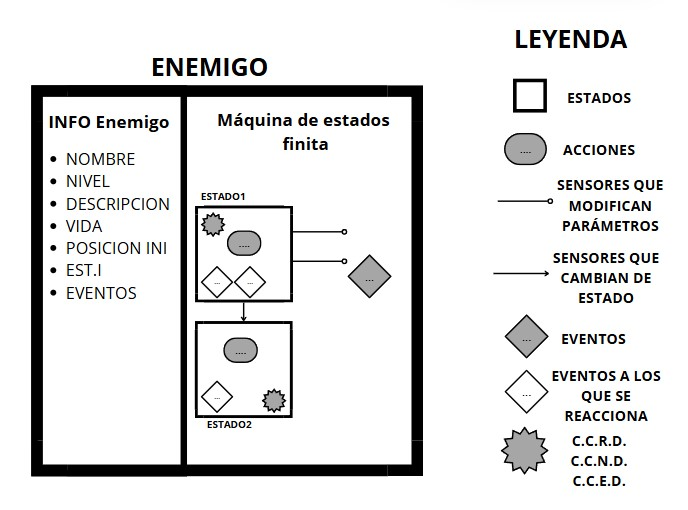
\includegraphics[width = 0.7\textwidth]{Imagenes/EnemigoGeneral.png}
	\caption{Enemigo General }
	\label{fig:EnemigoGeneral}
\end{figure}


\section{Ejemplos}
Aquí comienza la descripción del trabajo realizado. Se deben incluir tantos capítulos como sea necesario para describir de la manera más completa posible el trabajo que se ha llevado a cabo. Como muestra la figura \ref{fig:sampleImage}, está todo por hacer.


\begin{figure}[h]
	\centering
	
\includegraphics[width = 0.5\textwidth]{Imagenes/Vectorial/Todo.pdf}
	\caption{Ejemplo de imagen}
	\label{fig:sampleImage}
\end{figure}

Si te sirve de utilidad,  puedes incluir tablas para mostrar resultados, tal como se ve en la tabla \ref{tab:sampleTable}.


\begin{table}
	\centering
	\begin{tabular}{c|c|c}
		\textbf{Col 1} & \textbf{Col 2} & \textbf{Col 3} \\
		\hline\hline
		3 & 3.01 & 3.50\\
		6 & 2.12 & 4.40\\
		1 & 3.79 & 5.00\\
		2 & 4.88 & 5.30\\
		4 & 3.50 & 2.90\\
		5 & 7.40 & 4.70\\
		\hline
	\end{tabular}
	\caption{Tabla de ejemplo}
	\label{tab:sampleTable}
\end{table}
